
%(BEGIN_QUESTION)
% Copyright 2011, Tony R. Kuphaldt, released under the Creative Commons Attribution License (v 1.0)
% This means you may do almost anything with this work of mine, so long as you give me proper credit

This solar hot-air collector bank uses a variable-speed fan as the final control element, the temperature controller commanding the fan to blow air at different rates in order to maintain a relatively constant discharge temperature.  The hot air is being used to dehydrate food, and so precise temperature control is important:

$$\includegraphics[width=15.5cm]{i02474x01.eps}$$

The single most significant load in this process is sunlight intensity.  As the sun becomes covered by clouds, the heat output of the collector bank rapidly drops.  This, of course, affects the temperature of the air going to the food dryer.  Even though the feedback controller will eventually get the temperature back to setpoint, there are moments of deviation (error).

\vskip 10pt

Suppose a sunlight radiation transmitter (RT) were installed to detect incident sunlight intensity.  Sketch how this RT could be connected to the rest of the control system components to form a {\it feedforward} loop.

\vskip 10pt

Also, describe a real experiment you could do with this process to determine whether or not {\it dynamic compensation} (i.e. lead/lag) is necessary in the feedforward signal path for optimal control.

\vfil 

\underbar{file i02474}
\eject
%(END_QUESTION)





%(BEGIN_ANSWER)

This is a graded question -- no answers or hints given!

%(END_ANSWER)





%(BEGIN_NOTES)

As sunlight intensity increases, the fan must blow more and more air through the collectors in order to stabilize the temperature (more cool air in to balance more solar radiation in).  Thus, the RT needs to add to the TIC's output signal to pre-emptively drive the fan faster as radiation increases (note that gain and bias function blocks have been omitted from this control diagram for simplicity):

$$\includegraphics[width=15.5cm]{i02474x02.eps}$$

One could test for dynamic compensation suitability by first ``tuning'' the feedforward system as best as possible (with the feedback controller disabled so we're only looking at pure feedforward action), then monitoring the initial direction of deviation following a sunlight load change.  If a temporary swell or dip in temperature occurs after each load (sunlight) change, then we need dynamic compensation added to the feedforward signal.  

For example, suppose our test involved covering up one of the collectors with a blanket to temporarily block sunlight (i.e. a load change which would naturally tend to drive temperature down with the feedback controller in manual).  In a perfectly-proportioned feedforward system with no dynamic problems, the outlet temperature won't change at all.  However, in a perfectly-proportioned feedforward system with dynamic inequalities, what we will see is either a momentary dip in temperature followed by a rise back to setpoint, or a momentary rise in temperature followed by a fall back to setpoint.  If introducing a negative load change causes the temperature to first fall and then rise again, what it means is that the feedforward action is happening too late, and that we need to install a {\it lead} function in the feedforward loop to speed up the VFD's response.  If covering up one of the collectors with a blanket instead causes temperature to rise and then fall back to setpoint, it means our feedforward signal is having too quick of an effect and needs to be delayed using a {\it lag} function.

\vskip 10pt

Another way to test for whether or not we need dynamic compensation is to perform two tests and measure their relative response times: one test of fan-speed change, and another test whereby we throw a screen over the collectors to simulate a step-down in sunlight intensity.  With all controls in manual, we then plot the time delay responses following each change to see which cause has the most immediate effect on discharge temperature.

%INDEX% Control, strategies: feedforward with dynamic compensation (lead/lag)
%INDEX% Process: solar hot-air collector control system

%(END_NOTES)


